\documentclass[11pt,border=5pt]{standalone}
\usepackage{fontspec}
\setmainfont{cmunrm.otf}[BoldFont=cmunbx.otf,ItalicFont=cmunti.otf,BoldItalicFont=cmunbi.otf]
\usepackage{amsmath}
\usepackage{unicode-math}
\setmathfont{NewCMMath-Regular.otf}
\usepackage{tikz}
\usetikzlibrary{arrows.meta,patterns,angles,quotes}
\begin{document}
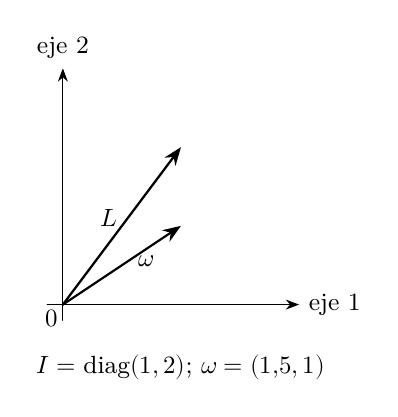
\begin{tikzpicture}[>=Stealth,font=\small,line cap=round,line join=round]
\draw[->,thin] (-0.2,0) -- (3,0) node[pos=1,right] {eje 1};
\draw[->,thin] (0,-0.2) -- (0,3) node[pos=1,above] {eje 2};
\node at (-0.14,-0.18) {$0$};
\draw[->,thick] (0,0) -- (1.5,1) node[pos=0.55,right] {$\omega$};
\draw[->,thick] (0,0) -- (1.5,2) node[pos=0.55,left] {$L$};
\node at (1.5,-0.8) {$I=\operatorname{diag}(1,2)$; $\omega=(1{,}5,1)$};

\end{tikzpicture}
\end{document}
